\documentclass[12pt, a4paper]{article}
\usepackage{enumerate}
\usepackage{amsmath}
\usepackage{amssymb}
\usepackage{blkarray}
\usepackage{geometry}
\usepackage{float}
\usepackage{graphicx}
\usepackage[linesnumbered, ruled]{algorithm2e}
\usepackage{forest}
\usepackage{diagbox}
\usepackage{cite}
\usepackage{url}
\usepackage{subfig}

\geometry{left = 2.0cm, right = 2.0cm}

\SetKwInOut{Input}{Input}
\SetKwInOut{Output}{Output}
\SetKwProg{Fn}{Function}{:}{end}
\SetKwFunction{TPS}{topological}

\title{
    \begin{figure}[H]
        \centering
        
\includegraphics[width=7cm, height=5cm]{AAA.png}
    \end{figure}
    VE477 Introduction to Algorithms\\ 
    Homework 3}
\author{Taoyue Xia, 518370910087}
\date{2021/10/18}

\begin{document}
\maketitle

\newpage

\section*{Ex. 1 --- Hamiltonian path}
\begin{enumerate}
    \item Depth-first search (DFS) is an algorithm for traversing or searching tree or graph data structures. 
          The algorithm starts at the root node, and explores as far as possible along each branch before backtracking or finding the exact route. 
          The pseudocode can be shown below:

          \begin{algorithm}
              \caption{Depth-first Search}
              \Input{A graph $G = \langle V, E\rangle$, $V$ for vertices, $E$ for edges}
              \Output{A tree of vertices reachable from}
              \SetKwFunction{DFS}{DFS}
              \BlankLine

              \Fn{\DFS{$G, v$}}{
                  $S \leftarrow$ a stack\;
                  push $v$ into $S$\;
                  \While{$S$ is not empty}{
                      $u \leftarrow S.pop()$\;
                      \If{$u$ is not visited}{
                          Label $u$ as visited\;
                          \For{each vertex $w$ adjacent to $u$}{
                              $S.push(w)$\;
                          }
                      }
                  }
              }
          \end{algorithm}

    \item Topological sort of a directed graph is a linear ordering of its vertices such that for every directed edge $uv$ from vertex $u$ to vertex $v$, 
          $u$ comes before $v$ in the ordering. A topological sort is possible if and only if the graph has no directed cycles, 
          which in other words, if it is a directed acyclic graph (DAG). Kahn's algorithm can explain topological sort clearly:

          \begin{algorithm}[!htb]
              \caption{Topological Sort (Kahn's Algorithm)}
              \Input{A directed graph $G = \langle V, E\rangle$}
              \Output{A list $L$ containing vertices in order after topological sort}
              \BlankLine
              \tcc{All vertices have an attribute $n$ for number of incoming edges}
              \Fn{\TPS{$G$}}{
                  $L \leftarrow$ an empty list which will contain sorted vertices\;
                  $S \leftarrow$ Queue of all vertices which initially have no incoming edge\;

                  \While{$S$ is not empty}{
                      $u \leftarrow S.pop()$\;
                      add $u$ to $L$\;
                      \For{all vertices $w$ which have an incoming edge from $u$}{

                          $w.n \leftarrow w.n - 1$\;
                          remove the edge $uw$ from $G$\;
                          \If{$w.n = 0$}{
                              push $w$ into $S$\;
                          }
                      }
                  }

                  \If{$G$ still has some edges}{
                      \KwRet{error} \tcp*{graph has circle, not DAG}
                  }
                  \KwRet{L}\;
              }
          \end{algorithm}
          \newpage
    \item For this problem, since a directed acyclic graph is given, we can use topological sort to sort the vertices in order. 
          After that, we can check whether there exists an edge for each two consecutive vertices in the list of sorted vertices. 
          If true, then there is a Hamiltonian path. If false, 
          then the answer would be no since we cannot go back in a Hamiltonian path in a DAG. 
          Since the time complexity of topological sort is $\mathcal{O}(V+E)$, 
          and the time complexity of check adjacency between consecutive vertices is $\mathcal{O}(V)$, 
          the total complexity of determining a Hamiltonian path is $\mathcal{O}(V+E)$.

          \begin{algorithm}[!htb]
              \caption{Hamiltonian Path Detection}
              \Input{A directed acyclic graph $G=\langle V, E \rangle$}
              \Output{a \textbf{flag} deciding whether the graph contains a Hamiltonian path or not}
              \SetKwFunction{HP}{Hamiltonian}
              \BlankLine
              \Fn{\HP{$G$}}{
                  $L \leftarrow$ \TPS{$G$}\;
                  \For{$i=0$ to $L.length - 2$}{
                      \If{no edge connecting $L[i]$ and $L[i+1]$}{
                          \KwRet{false}\;
                      }
                  }
                  \KwRet{true}\;
              }
          \end{algorithm}

    \newpage
    \item For the while loop in topological sort, it will loop $V$ times until all the vertices are visited. 
          For the for loop in it, since the graph is a DAG, all the edges are taken into account, 
          so the operation in for loop will be executed for at most $E$ times. Therefore, 
          the time complexity of topological sort is $\mathcal{O}(V+E)$. 
          Furthermore, the time complexity of check of edges between all consecutive vertices is $\mathcal{O}(V)$. 
          Therefore, the overall complexity is $\mathcal{O}(V+E)$.
    
    \item The problem belongs to $NP$ class.
\end{enumerate}

\section*{Ex. 2 --- Critical thinking}
\begin{enumerate}
    \item Firstly, by taking the logarithm of $n!$, we can calculate the time complexity of $\log(n!)$.
          \begin{align*}
              \log(n!) &= \log(1) + \log(2) + \cdots + \log n\\
                       &\leq \begin{matrix}
                           \underbrace{\log n + \log n + \cdots + \log n}\\ n
                       \end{matrix}\\
                       &= n\log n
          \end{align*}
          Therefore $\log(n!) = \mathcal{O}(n\log n)$. Furthermore, we can calculate whether it has a lower bound:
          \begin{align*}
              \log(n!) &= \log(1) + \log(2) + \cdots + \log n\\
                       &\geq \begin{matrix}\underbrace{\log(\lceil \frac{n}{2} \rceil) + \cdots + \log(\lceil \frac{n}{2} \rceil)}\\ n/2 \end{matrix}\\
                       &= \frac{n}{2}\log \frac{n}{2}\\
                       &= \frac{n}{2}(\log n - \log 2)\\
                       &= \frac{1}{2}n\log n - \frac{\log 2}{2} n\\
                       &= \Theta(n\log n)
          \end{align*}
          Therefore, we can prove that $\log(n!) = \Omega(n\log n)$. Therefore, $\log(n!) = \Theta(n\log n)$. 
          
          Then substitute $n$ with $\lceil \log n \rceil$, we can have:
          $$\log(\lceil \log n \rceil !) = \Theta(\lceil \log n \rceil \log(\lceil \log n \rceil)) = \Theta(\log n \cdot \log \log n)$$
          Suppose that $\lceil \log n \rceil !$ is bounded by a polynomial, then it means that $\log(\lceil \log n \rceil !) = \mathcal{O}(\log n)$. 
          However, $\log(\lceil \log n \rceil !) = \Theta(\log n \cdot \log \log n) \neq \mathcal{O}(\log n)$. Then it raises a contradiction.
          
          Therefore, $\lceil \log n \rceil !$ is not bounded by a polynomial.

    \item From slide c2, we have the definition of the iterated logarithm function $\log^*$ as:
          $$\log^* n = 
          \begin{cases}
              0 & \text{if } x \leq 1\\
              1 + \log^* \log n & \text{if } x > 1
          \end{cases}
          $$
          To make $\log \log^* n$ have sense, $n > 1$ should be satisfied. Then, we can express $\log \log^* n$ as:
          $$\log \log^* n = \log(1 + \log^* \log n)$$
          Set $\log^* \log n = t$. If a function $f(x)$ is asymptotically larger than $g(x)$, then it means that:
          $$\lim_{x\rightarrow \infty} \frac{f(x)}{g(x)} = \infty$$
          Therefore, let $f(t) = t = \log^* \log n$ and $g(t) = \log(1 + t)$, then set $h(t) = \frac{f(t)}{g(t)} = \frac{t}{\log(1 + t)}$.
          Then we can calculate the derivative of $h(t)$ as:
          $$\frac{dh(t)}{dt} = \frac{\log(1+t) - \frac{t}{1+t}}{\log^2(1+t)} \approx \frac{\log(1+t) - 1}{\log^2(1+t)}$$
          When $t$ is greater than 1, the derivative is greater than 0 and converge to $\frac{1}{\log(1+t)}$, which means that:
          $$\lim_{t\rightarrow \infty} \frac{f(t)}{g(t)} = \frac{\log^* log n}{\log \log^* n} = \infty$$
          when $t = \log^* \log n$. Proof done.

    \item The minimum number of weighing is 2, and the pseudocode is shown below
          
          \begin{algorithm}[!htb]
              \caption{8 balls weighing algorithm}
              \Input{8 balls $a_1\dots a_8$, and one ball is lighter while others are of same weight}
              \Output{The light ball}
              \SetKwFunction{BW}{weighBalls}
              \BlankLine

              \Fn{\BW{$a_1,\dots, a_8$}}{
                  Split the 8 balls into three groups $g_1 = (a_1,a_2,a_3)$, $g_2 = (a_4,a_5,a_6)$, $g_3 = (a_7,a_8)$\;
                  Weigh $g_1$ and $g_2$\;
                  \uIf{$weight(g_1) = weight(g_2)$}{
                      Weigh $a_7$ and $a_8$\;
                      \eIf{$weight(a_7) < weight(a_8)$}{\KwRet{$a_7$}}{\KwRet{$a_8$}\;}
                  }
                  \uElseIf{$weight(g_1) < weight(g_2)$}{
                      Weigh $a_1$ and $a_2$\;
                      \uIf{$weight(a_1) = weight(a_2)$}{\KwRet{$a_3$}\;}
                      \uElseIf{$weight(a_1) < weight(a_2)$}{\KwRet{$a_1$}\;}
                      \Else{\KwRet{$a_2$}\;}
                  }
                  \Else{Do the same procedure as for $g_1$\;}
              }
          \end{algorithm}
          From the above algorithm, we can optimize the weighing number to 2.
\end{enumerate}

\newpage

\section*{Ex. 3 --- Rubik’s Cube}
A Rubik's cube is a cube with six faces, each of different color, usually white, yellow, red, blue, green, orange. 
Then, each face is split into nine small squares, constructing three rows and three columns. 
Each face with one row can be rotated so that colors can be mixed, and create different permutations. 
The figure of a Rubik's cube (Fig.~\ref{fig:cube})

\begin{figure}[!htb]
    \centering
    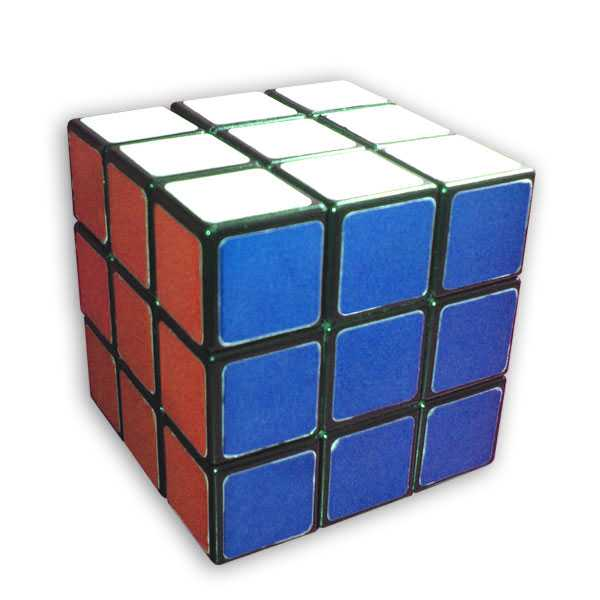
\includegraphics{cube}
    \caption{Rubik's cube}
    \label{fig:cube}
\end{figure}

\subsection*{Solution Algorithms}
To begin, first denote different symbols. Suppose that we face directly to a face of the cube. `$F$' means rotating the front face clockwise for $90^\circ$. 
Also, `$L$', `$R$', `$U$', `$D$' denote for rotating the left, right, upper and downside face clockwise for $90^\circ$. When adding a $'$ to the symbol, it means counterclockwise. 

\subsubsection*{Beginner's Method}
Then, referring to the figure below (Fig.~\ref{fig:solution1})

\begin{figure}[!htb]
    \centering
    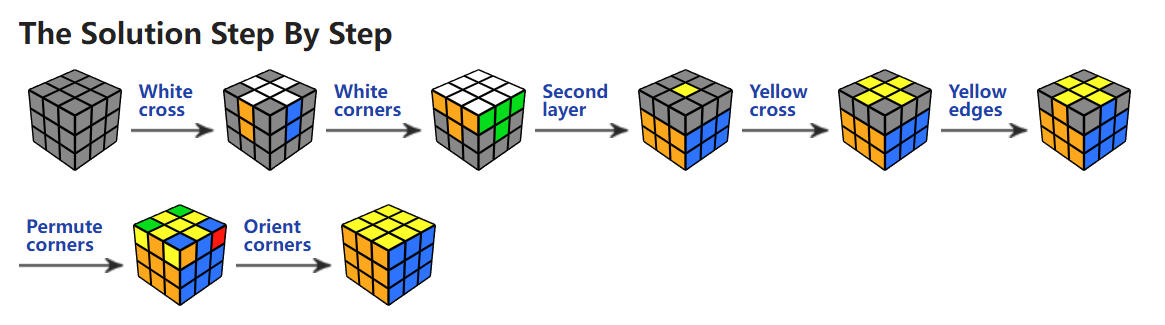
\includegraphics[width=14cm, height=4cm]{solution1}
    \caption{Solution for beginners.\cite{BeginnerMethod}}
    \label{fig:solution1}
\end{figure}

\begin{itemize}
    \item Firstly, build a white cross at the top layer, and fit each corner with the correct corresponding color to each face by using $R^\prime D^\prime R$, 
          then turn the top layer to the bottom.
    \item Then, to finish the second layer, in two different situations to replace a block with another, 
          we can use $U^\prime L^\prime U L U F U^\prime F^\prime$ or $URU^\prime R^\prime U^\prime F^\prime UF$.
    \item Then we can use the formula $FRUR^\prime U^\prime F^\prime$ to build a yellow cross in the top layer.
    \item After that, use $URU^\prime L^\prime U R^\prime U^\prime L$ to fit the corners.
    \item Finally, use $R^\prime D^\prime RD$ to get the cube all done.
\end{itemize}

\subsubsection*{Zbigniew Zborowski (ZZ) Method}
This method is originally proposed by Zbigniew Zborowski in 2006, which is comparatively faster than CFOP. Refer to the figure below (Fig.~\ref{fig:ZZ}):

\begin{figure}[!htb]
    \centering
    \subfloat[EOLine\label{fig:EOL}]{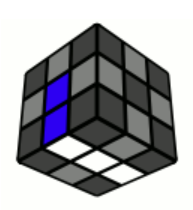
\includegraphics{EOLine}}
    \hspace{1cm}
    \subfloat[F2L\label{fig:F2L}]{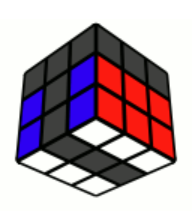
\includegraphics{F2L}}
    \hspace{1cm}
    \subfloat[LL\label{fig:LL}]{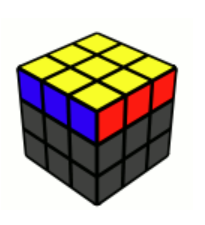
\includegraphics{LL}}
    \caption{Procedure of ZZ \cite{ZZ}}
    \label{fig:ZZ}
\end{figure}

\begin{itemize}
    \item First, one should fit a line at the bottom face of a cube, which is the EOLine part (Fig.~\ref{fig:EOL}).
    \item In the F2L stage, one should complete the first two layers by building two 1x2x3 blocks on either side of the Line made in the previous stage. 
          Since all edges are oriented, we just need $R$, $U$ and $L$ moves to complete the stage (Fig.~\ref{fig:F2L}).
    \item Finally, we can just simply apply methods done on the top layer, and will get the cube recovered (Fig.~\ref{fig:LL}).
\end{itemize}

\begin{thebibliography}{}
    \bibitem{BeginnerMethod} “How to solve the Rubik's Cube,” How to solve the Rubik's Cube - Beginners Method. [Online]. 
    Available: \url{https://ruwix.com/the-rubiks-cube/how-to-solve-the-rubiks-cube-beginners-method/}. [Accessed: 19-Oct-2021].
    \bibitem{ZZ} C. Rider, ZZ Method Tutorial. [Online]. Available: \url{http://cube.rider.biz/zz.php}. [Accessed: 19-Oct-2021]. 
\end{thebibliography}

\section*{Ex. 4 --- The $\mathcal{NP}$ class}
A problem is in $\mathcal{NP}$ if and only if given a certificate, the correctness of the answer can be determined with a polynomial time algorithm.
So considering the three problems:
\begin{enumerate}
    \item Finding a simple path is equivalent to find a Hamiltonian path. Set the certificate to be a simple path generated by topological sort, 
          It can be decided in polynomial time whether it is a simple path (according to Ex1.4). Therefore, it is $\mathcal{NP}$.
    \item Checking whether an integer is composite is in $\mathcal{NP}$ class. The certificate can be a small integer $i$, 
          suppose that the given integer is $n$, we can simply use Euclidean algorithm to check whether it is prime or not. 
    \item The vertex cover determination problem is also in $\mathcal{NP}$ class. Set the certificate to be a vertex cover of size $k$. 
          Then we just need to check in the given graph $G=\langle V, E\rangle$, for each $e = \langle u, v\rangle \in E$, 
          whether all $u$ and $v$ are in the vertex cover. It only takes time complexity of $\mathcal{O}(E)$.
\end{enumerate}

\section*{Ex. 5 --- \textit{PRIMES} in $\mathcal{P}$}
According to the \textbf{Prime Number Theorem}, given an integer $x$, there are about $\pi(x)$ primes less than it, where $\pi(x)$ is defined as:
$$\pi(x) \approx \frac{x}{\log x}$$
Trivial division can be simplified in the way that if $N$ is given to test its primality, 
we just need to take the primes less than or equal to$\sqrt{N}$ into account, since if we can find a prime factor larger than $\sqrt{N}$, 
you can always find a corresponding prime less than it. However, it doesn't mean that trivial division only have the time complexity of $\mathcal{O}(\sqrt{n})$. 

For example, let's assume that we need to check the primality of an integer $x$ with $n$ binary digits. 
Since we just need to take $\sqrt{x}$ into account, which is $2^{n/2}$, then according to the prime number theorem, we will have
$$\pi(2^{\frac{n}{2}}) = \frac{2^{\frac{n}{2}}}{\frac{n}{2} \log 2}$$
primes to be taken into account, will is not bounded in polynomial, but exponential.

Therefore, we can not prove that \textit{PRIMES} is in $\mathcal{P}$. Furthermore, one of the fastest algorithm to determine a number's primality, 
the quadratic sieve algorithm, can run with time complexity $e^{(1 + \mathcal{O}(1))\sqrt{\ln n \ln \ln n}}$, which is still not pseudo polynomial.


\end{document}